% "{'classe':('PSI','PT'),'chapitre':'oral_mt','type':('oral_mt'),'titre':'Train datterrissage d hélicoptère', 'source':'Banque PT -- SIA -- 2014','comp':(),'corrige':False}"
%\setchapterimage{bandeau}
\chapter*{Préparation Mines Telecom \\%\arabic{cptColle} \\ 
Train d'atterrissage d'hélicoptère \ifnormal $\star$ \else \fi \iftdifficile $\star\star\star$ \else \fi  -- 
\ifprof Corrigé \else Sujet \fi}
\addcontentsline{toc}{section}{Colle \arabic{cptColle} :
Train d'atterrissage d'hélicoptère \ifnormal $\star$ \else \fi \iftdifficile $\star\star\star$ \else \fi  -- 
\ifprof Corrigé \else Sujet \fi}

\iflivret \stepcounter{cptColle} \else
\ifprof  \stepcounter{cptColle} \else \fi
\fi

\setcounter{question}{0}
\marginnote{D'après concours Banque PT -- SIA -- 2014.}


\begin{marginfigure}
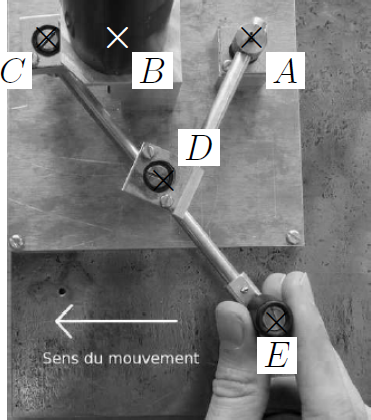
\includegraphics[width=\linewidth]{fig_00.png}
\caption{Appontage NH 90 \label{fig_sia2014_00}}
\end{marginfigure}


Le train d'atterrissage étudié est celui du NH 90, fondé sur un train à roues munies d'amortisseurs.  
Le train principal constitué de deux roues simples est installé dans le fuselage central et le train auxiliaire constitué de deux roues jumelées de direction dans la partie avant du fuselage figure \ref{fig_sia2014_00}. 
Des caissons permettent d'escamoter les trains d'atterrissage lors du vol. 

\begin{multicols}{2}
Une jambe du train principal est constituée de (figure \ref{fig_sia2014_01}) : 
\begin{itemize}
\item une roue avec un pneumatique;
\item un bras oscillant;
\item un vérin amortisseur : piston – cylindre;
\item un triangle anti-vrillage ou compas;
\item un vérin de rétraction : piston rétractable – cylindre. 
\end{itemize}

Le train auxiliaire situé à l'avant est constitué de (figure \ref{fig_sia2014_01}) : 
\begin{itemize}
\item deux roues jumelées;
\item un tube coulissant amortisseur;
\item un triangle anti-vrillage ou compas;
\item un support principal pivotant autour de l'axe vertical.
\end{itemize}
\end{multicols}

\begin{figure}[!h]
\centering
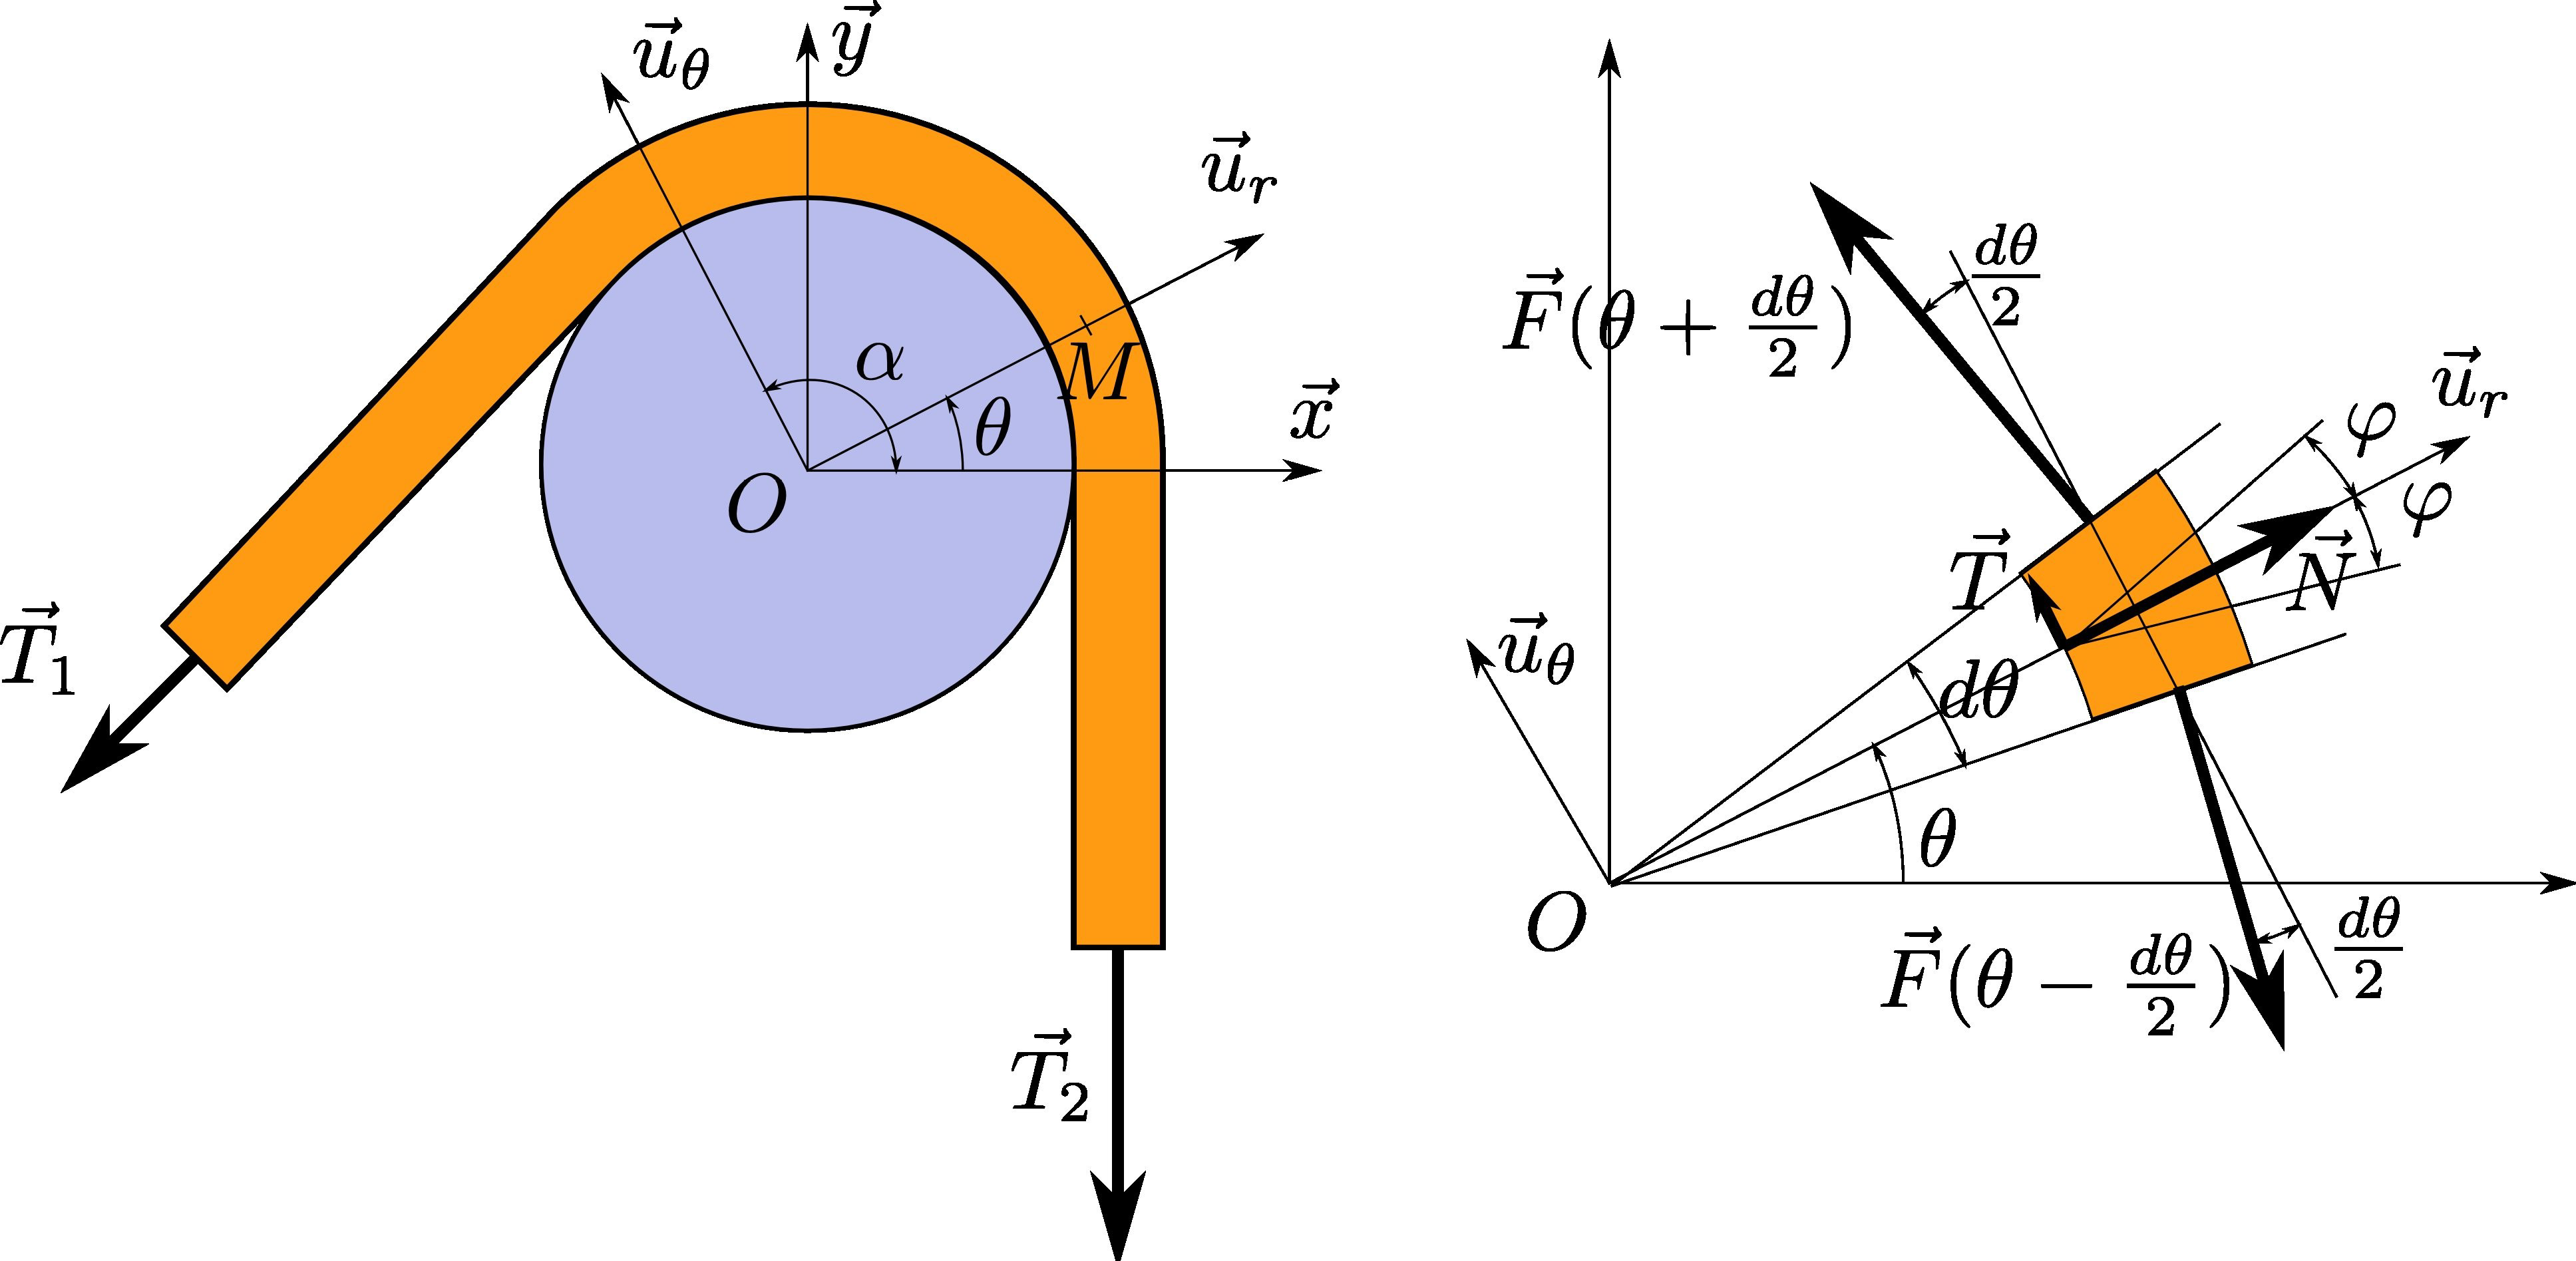
\includegraphics[width=\linewidth]{fig_01.png}
\caption{Maquette numérique des éléments du train d'atterrissage \label{fig_sia2014_01}}
\end{figure}

